%\documentclass[a0,landscape,posterdraft]{a0poster}
%\documentclass[a0b,landscape,final]{a0poster}
\documentclass[a0b,portrait,final]{a0poster}
\usepackage{colordvi,amsmath,epsfig,float,color,multicol,subfigure}
%\usepackage{grffile}
\usepackage[table]{xcolor}
\usepackage{pstricks,pst-node}
%\usepackage{txfonts}
\usepackage{tabularx}
\usepackage[framemethod=TikZ]{mdframed}
\usepackage{lipsum}

% landscape
% portrait
% a0b   ``DIN A0 big''. 915.1* 1200 mm 
% a0    ``DIN A0''.    839.6 * 1188.2 mm
% draft                 Gj�r om til A4 for testutskrift.
% final                 Gj�r at PS-fila blir i spesifisert st�rrelse;
%                       standard.
% ISO A0 size, 841 mm by 1189 mm.
% \tiny            12pt
% \scriptsize      14.4pt
% \footnotesize    17.28pt
% \small           20.74pt
% \normalsize      24.88pt
% \large           29.86pt
% \Large           35.83pt
% \LARGE           43pt
% \huge            51.6pt
% \Huge            61.92pt
% \veryHuge        74.3pt
% \VeryHuge        89.16pt
% \VERYHuge        107pt

% N�r du har kj�rt latex 'filnavn.tex', vil det dukke opp en fil til i
% katalogen; 'a0header.ps'. Denne filen m� ligge der n�r du kj�rer
% dvips.

%%%%%%%%%%%%%
%  Lengder: %
%%%%%%%%%%%%%

\addtolength{\textwidth}{-1cm}
\addtolength{\oddsidemargin}{0.2cm}

% Avstanden mellom kolonnene i multicolumn-mode
\setlength{\columnsep}{2.0cm}
\setlength{\parindent}{0cm}
\setlength{\parskip}{1.4ex}

%\pagestyle{empty}

% Setter standard skrifttype til � v�re 'phv'; Sans Serif.
\renewcommand{\familydefault}{phv}
% Setter standard skriftst�rrelse.
%renewcommand{\normalsize}{\huge}


\definecolor{DarkBlue}{rgb}{0.0470,0,0.5294}
\definecolor{rltred}{rgb}{0.75,0,0}
\definecolor{rltgreen}{rgb}{0.0470,0.5294,0}
\definecolor{rltblue}{rgb}{0,0,0.75}
\definecolor{DarkRed}{rgb}{0.75, 0, 0.09}
\definecolor{ForestGreen}{rgb}{0, 0.27, 0.13}
\definecolor{NapierGreen}{rgb}{0.16, 0.5, 0.0}
\definecolor{NavyBlue}{rgb}{0.0, 0.0, 0.5}
% see http://en.wikipedia.org/wiki/List_of_colors for RGB 

\makeatletter

\renewcommand{\section}{\@startsection
        {section}%                          % the name 
        {1}%                                % the level
        {0mm}%                              % the indent
        {-\baselineskip}%                   % the beforeskip
        {1mm}%                              % the afterskip
        {\LARGE\color{DarkBlue}\bfseries}}% % the style

\renewcommand{\subsection}{\@startsection
        {subsection}%                       % the name 
        {2}%                                % the level
        {1mm}%                              % the indent
        {-0.9\baselineskip}%                % the beforeskip
        {1mm}%                              % the afterskip
        {\Large\color{DarkRed}\bfseries}}% % the style
\renewcommand{\subsubsection}{\@startsection
        {subsubsection}%                    % the name 
        {3}%                                % the level
        {4mm}%                              % the indent
        {-0.7\baselineskip}%                % the beforeskip
        {1mm}%                              % the afterskip
        {\large\color{ForestGreen}\bfseries}}% % the style
\renewcommand{\paragraph}{\@startsection
        {paragraph}%                        % the name 
        {4}%                                % the level
        {6mm}%                              % the indent
        {-0.9\baselineskip}%                % the beforeskip
        {0mm}%                              % the afterskip
        {\large\color{NavyBlue}\slshape}}% % the style
\makeatother

\begin{document}
\begin{minipage}[t]{0.8\linewidth}
  {\veryHuge \textbf{Status Report of RAON Control System}}
  \\[1ex]
  \bigskip
     {\LARGE Soo Ryu} {\large \texttt{sryu@ibs.re.kr}}, 
     {J.H. Lee} {\texttt{jhlee@ibs.re.kr}},
     {S. Choi} {\texttt{choi3over4@ibs.re.kr}},
     {D. Jeon} {\texttt{jeond@ibs.re.kr}}.
     \hspace{8mm} \\
     \emph{\large   \textbf{R}are \textbf{I}sotope \textbf{S}cience \textbf{P}roject, \textbf{I}nstitute for \textbf{B}asic \textbf{S}cience, Daejeon, South Korea}
     \vspace{4mm}
\end{minipage}
\rput(0,-2){
\includegraphics[scale=0.8]{./images/RISPlogo.eps}}
\rput(9,-2){
\includegraphics[scale=0.56]{./images/IBSlogo.eps}}


\vspace{2cm}


\begin{multicols}{3}
\section*{Abstract}
The RAON~\cite{TSHOO:NIMB} is a new heavy ion accelerator under construction in South Korea,
which is to produce a variety of stable ion and rare isotope beams to
support various researches for the basic science and applied research applications.
To produce the isotopes to fulfill the requirements we have
planed the several modes of operation scheme which require fine-tuned
synchronous controls, asynchronous controls, or both among the accelerator complexes.
The basic idea and development progress of the control system
as well as the future plan are presented.


\section*{The RAON}
\vspace{2mm}
\begin{figure}[H]
  \centering
  \includegraphics[width=1\columnwidth]{./images/raon_cad_sketch2.eps}
\end{figure}
The RAON consists of both the 400 kW In-flight Fragmentation (IF) facility
and the 70 kW Isotope Separator On-Line (ISOL) facility.
The IF accelerator system is designed to produce stable ion beams with maximum energy
up to 200 MeV/u for uranium (600 MeV for proton).
The ISOL accelerator system delivers rare isotope beams with maximum energy of 18.5 MeV/u.
The two different systems should be operated both independently and concurrently with respect to the
user requirements, which is the unique feature of RAON accelerator system.

\section*{Requirements}
\begin{mdframed}[roundcorner=10pt]
\begin{itemize}
\item Integration of many different subsystems : \\ 
   RF system, beam diagnostics, power supply, vacuum control, beam line control, and machine protection
\item An exclusive operation two and more accelerator systems for two facilities : \\
   In-flight Fragmentations (IF) and Isotope On-Line (ISOL)
\item C.W. and pulsed beam operation
\item Beam off latency $<$ 50 $\mu$secs
\item Automation of most of subsystems and manual control of beam line elements
\item EPICS integration
\end{itemize}
\end{mdframed}


\section*{Architecture}
\begin{mdframed}[roundcorner=10pt]
\vspace{2mm}
\begin{figure}[H]
  \centering
  \includegraphics[width=1\columnwidth]{./images/ctrl_arch0.eps}
  %\caption{Overall architecture of the RAON control system}
  \label{fig:architecture}
\end{figure}

\begin{itemize}
\item Tightly integrated with the EPICS
\item Using two network grid : Timing event network and EPICS channel access (CA) network
\item The main building block is the control unit $\to$ for simplified and fast integration
\item CA network is linked to the database, HLA and EPICS control interface for users
\end{itemize}
\end{mdframed}

\subsection*{System Standards}
\begin{mdframed}[roundcorner=10pt]
\begin{itemize}
\item 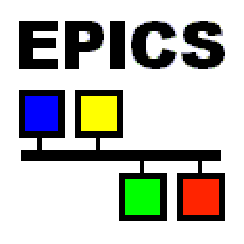
\includegraphics[width=0.01\textheight]{./images/epics_logo.eps}~ \textbf{EPICS}, All and Sundry systems ;-)
\item \includegraphics[width=0.01\textheight]{./images/debian_logo.eps} ~ Debian Linux for OS, VxWorks for RTOS
\item \includegraphics[width=0.01\textheight]{./images/postgresql_logo.eps}~ PostgreSQL for accelerator configuration
\item \includegraphics[width=0.009\textheight]{./images/subversion_logo.eps}~ SVN or \includegraphics[width=0.02\textheight]{./images/git_logo.eps}~for sources \& documents version control 
\item International / market  standard hardwares
\item 10 GB Ethernet backbone (1 GB for Usernet)
\end{itemize}
\end{mdframed}

\columnbreak


\subsection*{The Control Unit}
\begin{mdframed}[roundcorner=10pt]
\begin{figure}[H]
  \centering
  \includegraphics[width=1\columnwidth]{./images/ctrl_unit2.eps}
\end{figure}
\begin{itemize}
\item VME platform.
\item Consists of a SBC running with RTOS, EVR and I/O board.
\item EPICS I/O Controller controls the PLC and subsystem.
\item Ethernet connection with time stamps given by EVR.
\item PLC is the front-end interface to the subsystems.
\end{itemize}
\end{mdframed}


% the EPICS IOC via Ethernet connection with time stamps given by EVR.
% In addition to the I/O board, a commercial/homemade FPGA board will be used for the signal processing.
% The PLC will be used for the front-end interface to the subsystems.
% The several vendors for PLC providing robust products, such as Allen-Bradley and SIEMENS, are considered.
% In addition the domestic PLC providers, such as LSIS~\cite{lsis}, are also considered in order to reduce the price.

\subsection*{Timing system \& Machine protection}

\begin{mdframed}[roundcorner=10pt]
\begin{itemize}
\item Timing system requires :
  \begin{itemize}
  \item[-] low latency, jitter in fs level.
  \item[-] deterministic operation.
  \item[-] high speed signal processing.
  \item[-] identifying a bunch.
%for RF phase and machine control, and low level RF feedback.
\end{itemize}

\item We will use :
  \begin{itemize}
  \item[-] MRF EVG/EVR hardwares~\cite{MRF}
  \item[-] Libera BPM products~\cite{LIBERABPM}
  \end{itemize}

\item We are considering to :
  \begin{itemize}
  \item[-] use White Rabit for timing system \cite{WR}.
  \item[-] develope homemade BPM with domestic company.
  \end{itemize}
\end{itemize}
\end{mdframed}

\begin{mdframed}[roundcorner=10pt]
\begin{figure}[H]
  \centering
  \includegraphics[width=1\columnwidth]{./images/safety_system2.eps}
\end{figure}

\begin{itemize}
\item Interlock controller : use PLC (S7, AB, LSIS~\cite{lsis})
\item Integrated with timing system using FPGA based controller.
\item Still need idea for more complicated system.
\end{itemize}
\end{mdframed}

%\begin{center}
%\rowcolors{1}{blue!20}{blue!6}
%\begin{tabularx}{0.934\columnwidth }{{ >{\hsize =0.30\hsize }X  >{\hsize =1.70\hsize }X}}
%\textbf{TDR}    & Technical Design Report \newline - build a testbed \\
%\textbf{LCS}    & Local Control System \newline  - build/test a prototype LCS for a dummy system\\
%\textbf{CCS I}  & Central Control System Part I\newline - design/test CCS from LCS and support subsystem prototypes\\
%\textbf{OPTIM}  & Optimization and Performance test \newline - check possible bottleneck for all connections\\
%\textbf{CCS II} & Central Control System  Part II \newline - setup the main control room\\
%\textbf{COMM}   & Commissioning \newline - maybe 24/7 works
%\end{tabularx}
%\end{center}


%\section*{Data management \& \\ System integration tool}

\subsection*{Database}
\begin{mdframed}[roundcorner=10pt]
\begin{itemize}
\item Data Archieving : PV, HW/SW configuration, A/D signals, Logging.
\item Documentaion and version control.
\item DAQ and pre-processing : BPM and RF related data. 
\item Use open-source based programs : Channel Archiever with PostgreSQL.
\item Develope an archiving framework dedicated to RAON.
\end{itemize}
\end{mdframed}

\subsection*{User Interface / High Level Application}
\begin{mdframed}[roundcorner=10pt]
\begin{itemize}
\item Intuitive, Comprehensive.
\item Applying existing EPICS CA Clients : EDM, MEDM, StripTool, CSS.
\item Developing an UI envrionment dedicated to RAON using existing tools :
\begin{itemize}
\item[-] C/C++  : EPICS Qt
\item[-] JAVA   : JCA 
\item[-] Python : Cothread
\item[-] LabView : CaLab
\end{itemize}
\item SNS, CSNS, ESS, GANIL, TRIUMF, and FRIB use/plan to use the XAL~\cite{XAL}.
\item Consider to use XAL and join OpenXAL~\cite{OPENXAL} project.
\end{itemize}
\end{mdframed}

\columnbreak

%Since XAL~\cite{XAL} has proved its usability and stability at Spallation Neutron Source (SNS) for several years,
%many recent accelerator projects such as CSNS, ESS, GANIL, TRIUMF, and FRIB, adopt
%this framework for building their own high level programming infrastructure.
%Moreover, the RAON control system demands the capabilities provided by XAL from the beginning of
%beam commissioning to the actual operation.
%Thus, the OpenXAL~\cite{OPENXAL}, an open source version of development framework,
%is selected as a high level application solution of the RAON control system.
%Using the object-oriented feature of Java,
%a hierarchical structure of the accelerator components will be modeled.
%Since there are many works to do, however, the international co-work is necessary.


\section*{Status}

\subsection*{The control unit for timing system}
\begin{mdframed}[roundcorner=10pt]
\begin{figure}[H]
\centering
  \includegraphics[width=.9\columnwidth]{./images/timing2.eps}
%\caption{The timing system prototyping}
\label{fig:timing_prototype}
\end{figure}
\begin{itemize}
\item Two test VME crates consisting of EVG, EVR, and MVME6100 with VxWorks 6.9.
\item Connected via EPICS channel access using fiber cables for event network.
\item Test : jitter, delay time, latency.
\item It will be used to test injector and superconducting LINAC system.
\item The international bidding for prototyping is under way in parallel.
\end{itemize}
\end{mdframed}



\subsection*{The vacuum control system}

\begin{mdframed}[roundcorner=10pt]
\begin{figure}[H]
\centering
  \includegraphics[width=1\columnwidth]{./images/testbed_vacuum.eps}
%\caption{The vacuum control system}
\label{fig:vacuum_control}
\end{figure}
\begin{itemize}
\item A testbed for the vacuum control system is being developed with a domestic company.
\item The vacuum system controlled by PLC will be integrated with EPICS and be used for the test facilities.
\end{itemize}
\end{mdframed}

\subsection*{Naming convention}
\begin{mdframed}[roundcorner=10pt]
\begin{itemize}
\item Important for the system integration
\item Should be comprehensive to user and maintainer.
\end{itemize}
%The naming convention is important for the system integration with EPICS,
%because it is related not only to the user comprehension but also
%to the issues on network and hardware I/O and data management.
A primitive naming convention study is done and shown as following:
%and the structure is followed by EPICS style~\cite{esstechnote0005}.
\begin{displaymath}
\textrm{DDDDIII-SSSS:TTTT.XXXX},
\end{displaymath}
where DDDDIII is a device identifier, SSSS is a system name, TTTT is the signal name
followed by the EPICS DB convention, and XXXX is the signal suffix.
This naming convention is not fixed but being improved upon the user's request.
\end{mdframed}



\section*{Summary \& Outlook}
\begin{mdframed}[roundcorner=10pt]
The goal of RAON control system is to provide good environment to operate the IF and ISOL accelerator systems.
The notion of system architecture and the control unit are being developed.
The development of a testbed for vacuum control system and a prototype of timing system together with MPS are also proceeding.
Since a test facility for injector and linear accelerator is planned to be finished in next year, the two prototyping of control and timing system will be tested and evaluated.
In addition the engineering design of central control system will start soon.
\end{mdframed}

\section*{Acknowledgement}
This work is supported by the Rare Isotope Science Project funded by 
Ministry of Science, ICT and Future Planning (MSIP) 
and National Research Foundation (NRF) of KOREA.

\begin{thebibliography}{9}   % Use for  1-9  references
%\begin{thebibliography}{99} % Use for 10-99 references

\bibitem{TSHOO:NIMB} Y.~K.~Kwon, {\it et. al},``Status of Rare Isotope Science Project in Korea'',
 Few-Body Syst 54, 961-966, (2013).
%\bibitem{TSHOO:NIMB} K.~Tshoo, {\it et. al},``Experimental systems overview of the Rare Isotope Science Project in Korea'',
%Nucl. Inst. Meth. Phys. B. (2013)

\bibitem{lsis}
LSIS~ PLC solutions, \texttt{http://www.lsis.co.kr/ls/\\ product/product\_cate02.asp?cate01=A03\&cate02=001}

\bibitem{MRF}
Event system by Micro-Research Finland Oy, \\ \texttt{http://www.mrf.fi}

\bibitem{LIBERABPM}
BPM phase \& position processor, \texttt{http://www.i-tech.si}

\bibitem{WR}
M. Lipinski, J. Serrano, T. Wlostowski, and C. Prados, ``Reliability in a White Rabbit Network'',
ICALEPCS'11, WEMMU007 (2011).

\bibitem{XAL}
J. Galambos, {\it et. al.}, ``SNS Application Programming Environment'', EPAC 2002, Paris, France (2002).

\bibitem{OPENXAL}
Open XAL project, \texttt{http://xaldev.sourceforge.net}

%\bibitem{esstechnote0005}
%G. Trahern, ``ESS Naming Convention'', ESS AD Technical Note.


\end{thebibliography}




\end{multicols}




%\vspace{13mm}

%\begin{minipage}[b]{1\linewidth}

%\section*{RAON Major Operations Modes}
%\vspace{2mm}
%\begin{figure}[H]
 % \includegraphics[width=0.99\columnwidth]{./images/raon_all_modes.eps}
%\end{figure}

%\end{minipage}





\end{document}

